\subsection{Teknologier til visualisering}
Vi ser en tydelig mulighed for at assistere forbrugere med at træffe et valg, når det kommer til køb af varer på nettet. For at undersøge hvilke teknologier, der kan anvendes til visualisering, er der i dette afsnit en række teknologier og metoder, som alle er relevante i forhold til at visualisere en lampe. Teknologierne er udvalgt på baggrund af diskussion i gruppen, hvor mindre relevante teknologier, som f.eks. 3D-print blev fravalgt. Formålet med afsnittet er, at få en forståelse af hvilke teknologier der allerede eksisterer inden for visualisering, og finde ud af hvilke metoder, der er bedst i forhold til visualisering af lamper for brugere der handler via internettet. De enkelte teknologier vurderes på baggrund af teknologiens fordele og ulemper i forhold til at besvare den endelige problemformulering.

\subsubsection{Digitale billeder taget med et fysisk kamera}
Som beskrevet under afsnit \ref{sec:ehandel}, benytter e-butikker, sig ofte af billeder til at vise kunden deres varer over internettet. Et eksempel på dette er vist på figur \ref{fig:e_handel_lampebilleder}.

\begin{figure}[H]
    \centering
    \fbox{\rule{\textwidth}{5cm}}
    \caption{Billeder af lamper på e-butikken somelampstore.what}
    \label{fig:e_handel_lampebilleder}
\end{figure} 

I det viste tilfælde er visualiseringen skabt ved at tage billeder af lamperne med et kamera fra en bestemt vinkel, i en kontekst, der typisk hænger sammen med lampetypen. 

Fordelen ved denne type af visualisering er, at den giver et virkelighedstro billede af, hvordan lampen ser ud i den kontekst, som billedet er taget i. Ulempen er, at der ofte kun er et begrænset antal billeder til rådighed, hvilket kan medføre, at forbrugeren ikke kan se lampen fra alle vinkler og på den måde ikke kan visualisere lampen for sig. Derudover kan det være svært, at se hvordan lyset udbreder sig fra lampen, da dette til dels afhænger af hvilken vinkel man ser lampen fra. 

Herudfra kan man kortfattet sige, at visualisering af lamper gennem billeder, taget med et fysisk kamera, giver et realistisk billede af lampen, men kun i den kontekst og vinkel billedet er taget i. 


\subsubsection{Augmented Reality App}
Augmented Reality er en teknologi der kan sætte virtuelle objekter ind i en virkelig kontekst. Derudover har man mulighed for at interagere med objektet i real tid. 
Denne metode bruger producenten "Artemides" i deres Augmented Reality App. Appen virker ved, at man scanner et logo fra et fysisk lampekatalog, hvorefter en givet lampe vil vise sig på logoets plads. Det er herefter muligt at flytte kataloget for, at se lampen i forskellige kontekster. Derudover har man mulighed for at rotere i alle vinkler samt tænde og slukke for lampens pære. 
Fordelene ved appen er, at brugeren har mulighed for selv at vælge hvilken lampe de vil se i sin egen kontekst, samt interagere med lampen. Herved har brugeren mulighed for, at se præcist hvordan lampen ser ud. 
Ulemperne ved appen er, at den ikke visualisere lampens belysning særlig godt, da dens første priotet er at visualisere selve lampens design. Derudover er det ikke muligt at visualisere lamper i en kontekst, hvis man ikke har den nødvendige bog som indeholder logoer over de forskellige lampedesigns i 3D. En anden ulempe er, at lampeudvalget er meget begrænset da det kun er udvalgte produkter fra "Artemides" som kan visualiseres. 
Nedenstående figur viser "Artemides" brugervejledning til appen.

\begin{figure}[H]
    \centering
    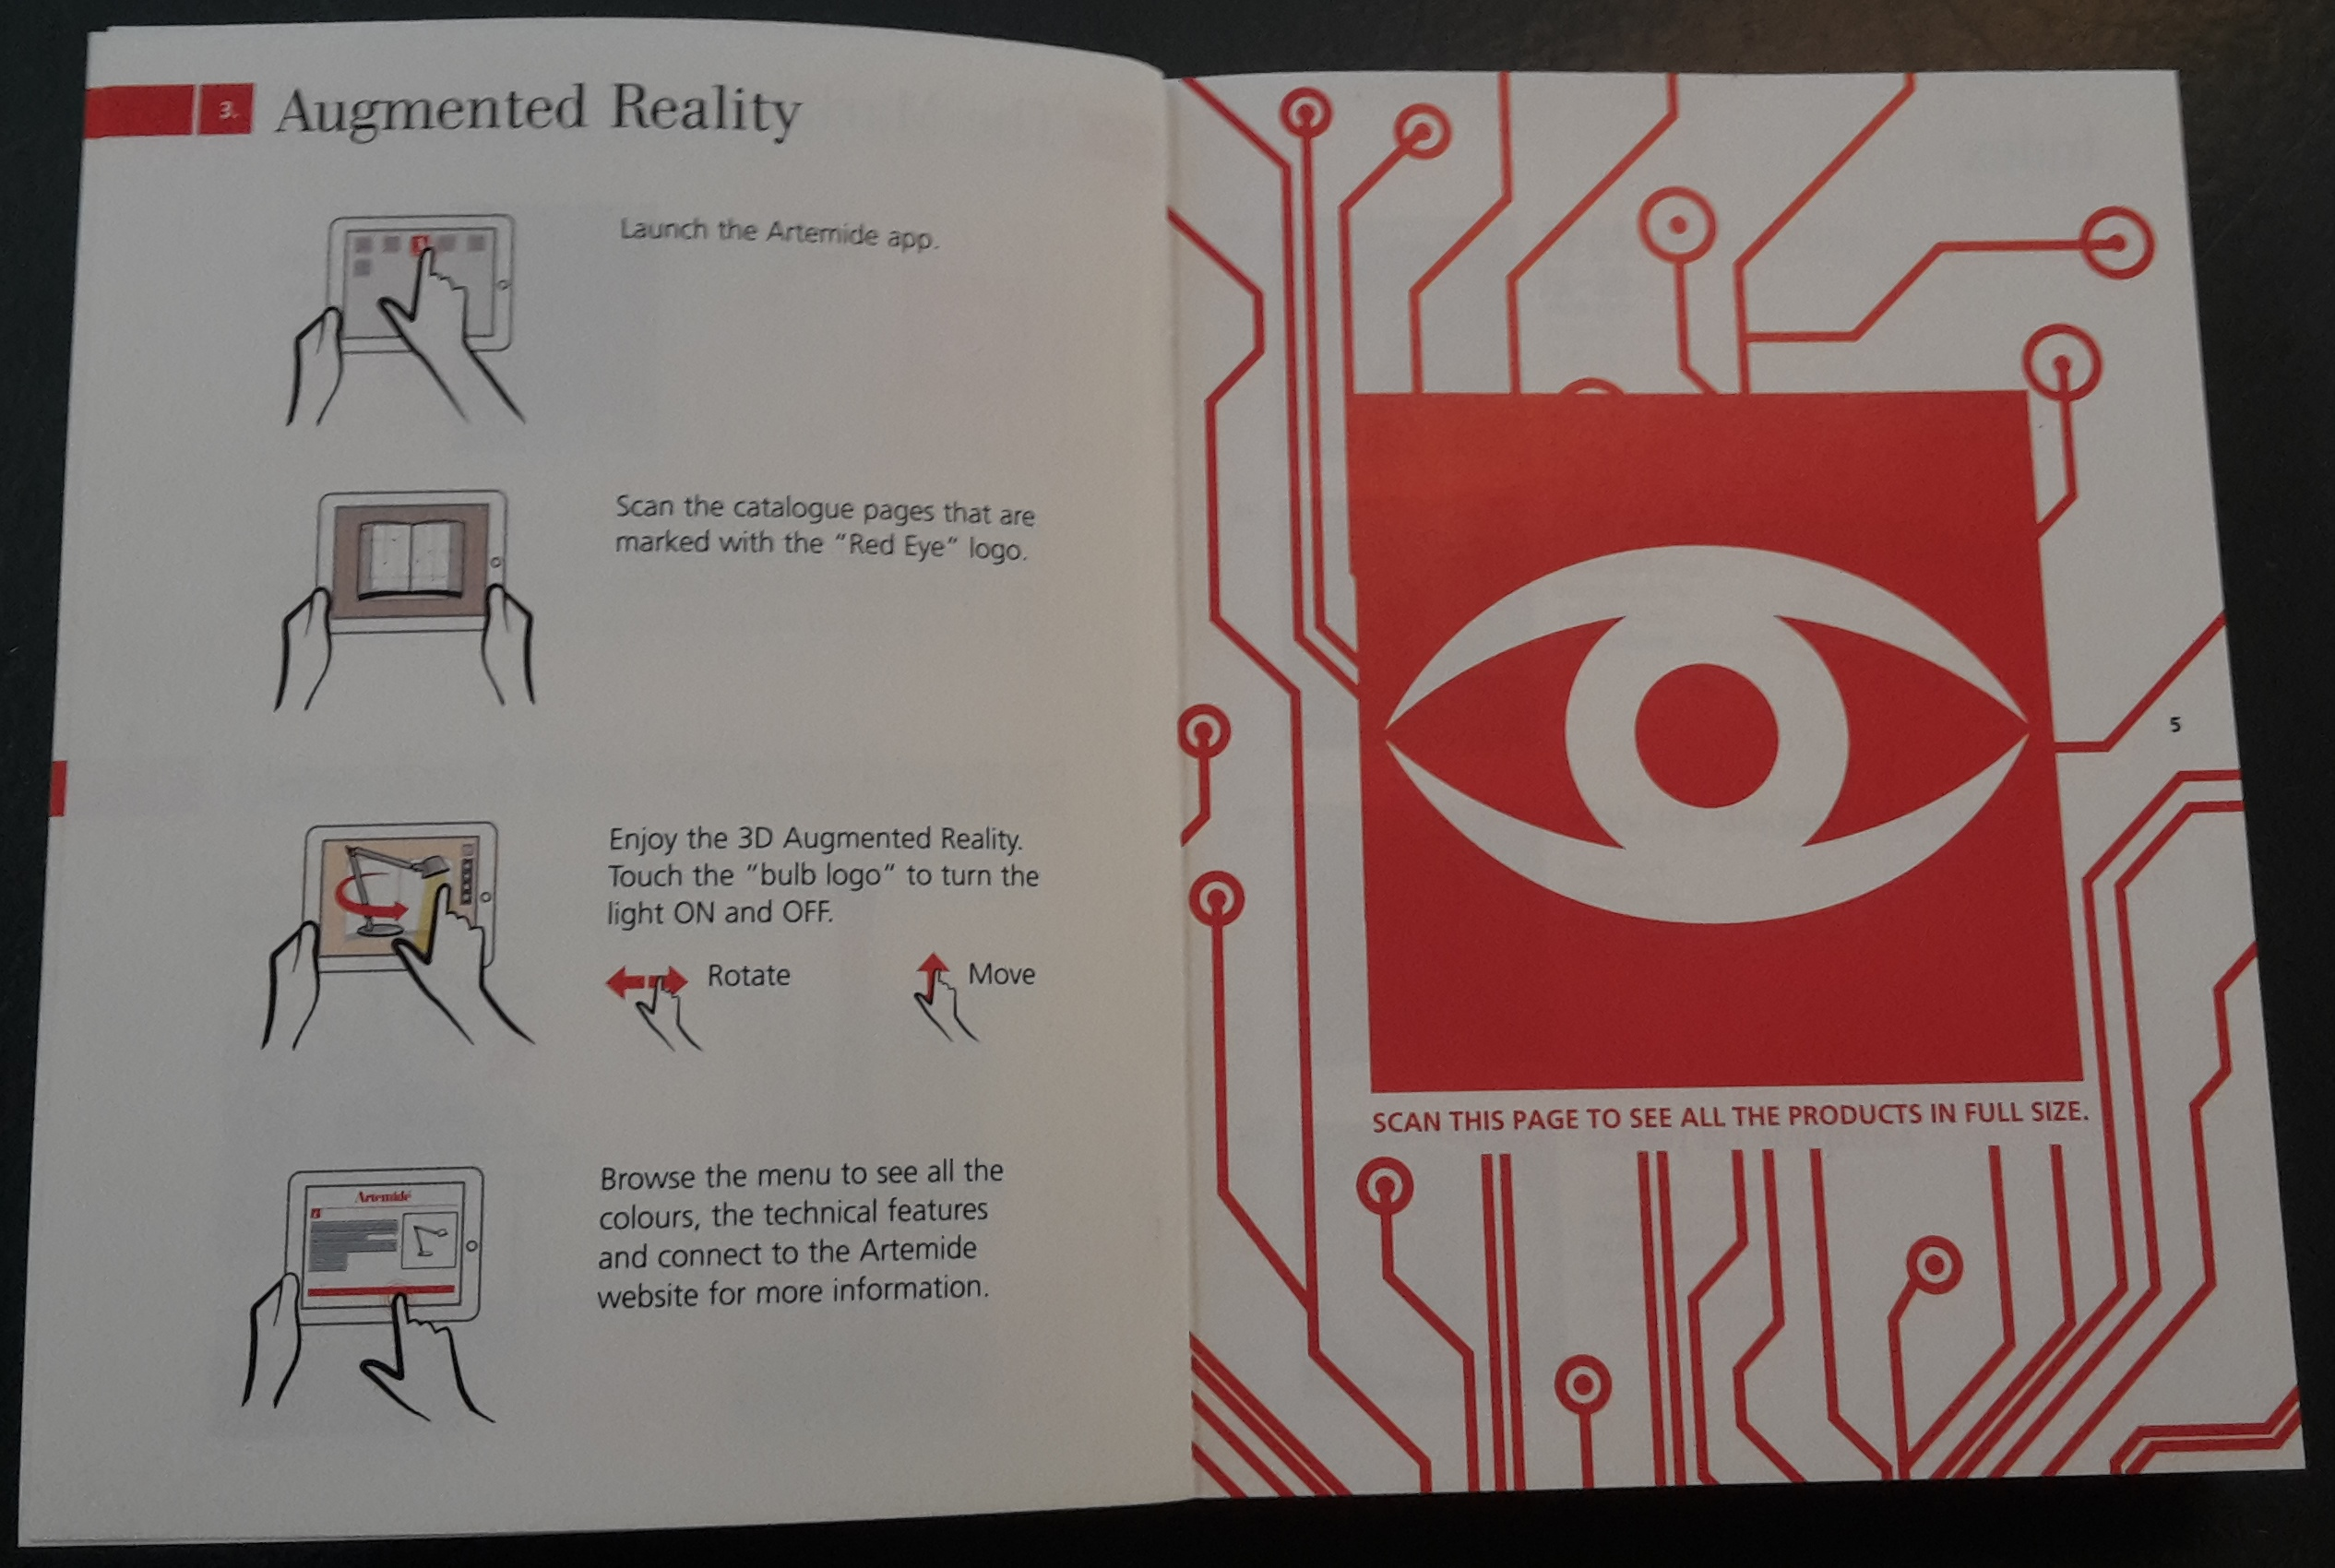
\includegraphics[width=10cm]{augmented_reality_artemides}
    \caption{Brugervejledning fra Artemides augmented reality.}
    \label{fig:augmented_reality_artemides}
\end{figure} 


\subsubsection{Computergrafik}
\label{sec:computergrafik}
I computergrafik, er en 3D model, en beskrivelse af objekters form og materiale \cite{computergrafik_introduktion}. Computergrafiske metoder kan bruges til at simulere, hvordan lys interagere med modellen og på den måde tegne et billede af modellen. Der eksisterer forskellige computergrafiske metoder, flere af hvilke kan bruges sammen med andre for, at opnå et mere realistisk eller effektivt resultat. Der er allerede værktøjer, som kan visualisere produkter til salg på websites som f.eks.\ Cylindo \cite{Cylindo}. Vi har ikke kendskab til at andre specialiserer sig, eller markedsfører sig på nuværende tidspunkt med deres kompetencer med fokus på visualisering af lampers belysning. Derfor er der herunder beskrivelse af to af de mest anvende metoder inden for computergrafik.

\paragraph{Rasterisering}
er en metode til at visualisere miljøer med høj aktiv brugerinteraktion som f.eks.\ computerspil \cite{rastarization}. Metoden virker ved rent matematisk at projektere modellen på et billedplan som repræsentere skærmen \cite{rastarization}. Fordelen ved rasterisering er at disse projektioner, kan foretages meget hurtigt af computerens grafikkort, som er bygget specielt til formålet \cite{rastarization}. Dette kan dog mindske fleksibiliteten, og muligheden for mere avancerede visualisering, hvor der kræves refleksioner og refraktioner af lys, som ikke passer ind i den proces (graphics pipeline \cite{rastarization}, som de enkelte grafikkort danner billeder ud fra). 

\paragraph{Ray tracing} [DER MANGLER KILDER TIL PÅSTANDE I DETTE AFSNIT]() forsøger, nøjagtigt at simulere lys i et virtuelt miljø, i modsætning til rasterisering hvor hastighed er den primære faktor. Raytracing bygger fundamentalt på at følge lysstråler og bygge en model for hvordan lysstrålerne interagere med forskellige objekter og materialer \cite{raytracing_for_begyndere}. 

I forhold til rasterisering, tager det længere tid at tegne, men komplekse lysfænomener som refleksioner og lys forvrængninger igennem semitransparante medier som vand(kaldet refraktion) er simple at beskrive for en raytracing algoritme, som kan tegne disse med realistisk precision. Nogle fænomener som bløde skygger kan også beskrives men jo flere typer fænomener og jo større realisme der kræves des længere tid tager det at tegne et billede, men raytracing tillader stor fleksibilitet.

\subsubsection*{Opsummering}
Ud fra ovenstående afsnit er der udledt følgende fordele og ulemper for de enkelte teknologier.
\begin{table}[h!]
  \centering
  
\center
    \begin{tabular}{ | p{3cm} | p{5cm} | p{5cm} |}
    
    \hline
    Teknologi & Fordele & Ulemper \\ \hline
    Kamerabilleder & Realistisk visualisering. & Tidskrævende. Begrænset kombinationer af lampen, synsvinkel, farvetemperatur og kontekst. \\ \hline
    Augmented Reality & Lampen er i konteksten & Manglende realisme af lampens belysning \\ \hline
   Computergrafik & Nemt at integrere på lampebtuikker hjemmesider. Kan opnå høj realisme af lampen og dens belysning. Nemt at ændre vinkel, farvetemperatur og kontekst hvorfra lampen visualiseres. & Kræver 3D-model af lampen og konteksten. Kræver meget computerkraft ved høj realisme. \\ \hline
    \end{tabular}
\caption{Viser fordele og ulemper ved de tre teknologier til visualisering.}
\label{tab:fordele_ulemper_teknologier}
\end{table}

På baggrund af fordele og ulemper vist i tabel \ref{tab:fordele_ulemper_teknologier} har gruppen valgt at arbejde videre med computergrafik, herunder raytracing, som teknologi til visualisering. Dette skyldes at raytracing, til dels kan visualisere lamper og deres belysning, men også give muligheden for at skifte lampe,  farvetemperatur, synsvinkel og kontekst uden at hverken producenten, e-butikken eller brugeren skal udføre ekstra arbejde. 



